% !TEX spellcheck = en_US
% !TEX spellcheck = LaTeX

\documentclass[letterpaper,english,10pt]{article}
\usepackage{%
	amsfonts,%
	amsmath,%	
	amssymb,%
	amsthm,%
	babel,%
	bbm,%
	%biblatex,%
	caption,%
	centernot,%
	color,%
	enumerate,%
	%enumitem,%
	epsfig,%
	epstopdf,%
	etex,%
	fancybox,%
	framed,%
	fullpage,%
	%geometry,%
	graphicx,%
	hyperref,%
	latexsym,%
	mathptmx,%
	mathtools,%
	multicol,%
	pgf,%
	pgfplots,%
	pgfplotstable,%
	pgfpages,%
	proof,%
	psfrag,%
	%subfigure,%	
	tikz,%
	times,%
	ulem,%
	url,%
	xcolor,%
	mathpazo
}

\definecolor{shadecolor}{gray}{.95}%{rgb}{1,0,0}
\usepackage[margin=1in,top=0.75in]{geometry}
\usepackage[mathscr]{eucal}
\usepgflibrary{shapes}
\usepgfplotslibrary{fillbetween}
\usetikzlibrary{%
  arrows,%
  backgrounds,%
  chains,%
  decorations.pathmorphing,% /pgf/decoration/random steps | erste Graphik
  decorations.text,% 
  matrix,%
  positioning,% wg. " of "
  fit,%
  patterns,%
  petri,%
  plotmarks,%
  scopes,%
  shadows,%
  shapes.misc,% wg. rounded rectangle
  shapes.arrows,%
  shapes.callouts,%
  shapes%
}

%\pgfplotsset{compat=newest} %<------ Here
\pgfplotsset{compat=1.11} %<------ Or use this one

\theoremstyle{plain}
\newtheorem{thm}{Theorem}[section]
\newtheorem{lem}[thm]{Lemma}
\newtheorem{prop}[thm]{Proposition}
\newtheorem{cor}[thm]{Corollary}
\newtheorem{clm}[thm]{Claim}

\theoremstyle{definition}
\newtheorem{axiom}[thm]{Axiom}
\newtheorem{defn}[thm]{Definition}
\newtheorem{conj}[thm]{Conjecture}
\newtheorem{exmp}[thm]{Example}
\newtheorem{exerc}[thm]{Exercise}
\newtheorem{assum}[thm]{Assumptions}

\theoremstyle{remark}
\newtheorem{rem}[thm]{Remark}
\newtheorem{note}[thm]{Note}

\newcommand{\Cov}{\operatorname{Cov}}
%\newcommand{\det}{\operatorname{det}}
\newcommand{\Real}{\mathbb{R}}
\newcommand{\tr}{\operatorname{tr}}
%\newcommand{\Var}{\operatorname{Var}}

\DeclareMathOperator{\sign}{sign}
%\renewcommand{\proof}[1]{\begin{proof}#1\end{proof}}
\newcommand{\EQ}[1]{\begin{equation*}#1\end{equation*}}
\newcommand{\EQN}[1]{\begin{equation}#1\end{equation}}
\newcommand{\eq}[1]{\begin{align*}#1\end{align*}}
\newcommand{\meq}[2]{\begin{xalignat*}{#1}#2\end{xalignat*}}
\newcommand{\norm}[1]{\left\lVert#1\right\rVert}
\newcommand{\abs}[1]{\left\lvert#1\right\rvert}
\newcommand{\expect}[1]{\mathbb{E}\left[{#1}\right]}
\newcommand{\prob}[1]{\mathbb{P}\left[{#1}\right]}
\newcommand{\given}{\; \big\vert \;} 
\newcommand{\set}[1]{\left\{#1\right\}} 
\newcommand{\indicator}[1]{\mathbb{1}_{\set{#1}}} 
\newcommand{\inner}[1]{\left\langle#1\right\rangle}
\newcommand{\red}[1]{\textcolor{red}{#1}} 
\newcommand{\E}[1]{\mathbb{E}\left[#1\right]}
\newcommand{\Var}[1]{\operatorname{Var}\left[#1\right]}

\newcommand{\D}{\mathbb{D}}
%\newcommand{\E}{\mathbb{E}}
\newcommand{\N}{\mathbb{N}}
\renewcommand{\P}{\mathbb{P}}
\newcommand{\Q}{\mathbb{Q}}
\newcommand{\R}{\mathbb{R}}
\newcommand{\Z}{\mathbb{Z}}

\newcommand{\bU}{\mathbf{1}}
\newcommand{\bx}{\mathbf{x}}

\newcommand{\cB}{\mathcal{B}}
\newcommand{\cC}{\mathcal{C}}
\newcommand{\cD}{\mathcal{D}}
\newcommand{\cF}{\mathcal{F}}
\newcommand{\cG}{\mathcal{G}}
\newcommand{\cH}{\mathcal{H}}
\newcommand{\cO}{\mathcal{O}}
\newcommand{\cT}{\mathcal{T}}
\newcommand{\cX}{\mathcal{X}}
\newcommand{\cY}{\mathcal{Y}}

\newcommand{\sA}{\mathscr{A}}
\newcommand{\sB}{\mathscr{B}}
\newcommand{\sC}{\mathscr{C}}
\newcommand{\sD}{\mathscr{D}}
\newcommand{\sE}{\mathscr{E}}
\newcommand{\sF}{\mathscr{F}}
\newcommand{\sG}{\mathscr{G}}
\newcommand{\sH}{\mathscr{H}}
\newcommand{\sL}{\mathscr{L}}
\newcommand{\dO}{\mathscr{O}}
\newcommand{\sS}{\mathscr{S}}
\newcommand{\sT}{\mathscr{T}}
\newcommand{\sX}{\mathscr{X}}
\newcommand{\sY}{\mathscr{Y}}
\newcommand{\sZ}{\mathscr{Z}}

% Debug
\newcommand{\todo}[1]{\begin{color}{blue}{{\bf~[TODO:~#1]}}\end{color}}

% a few handy macros

\renewcommand{\le}{\leqslant}
\renewcommand{\ge}{\geqslant}
\newcommand\matlab{{\sc matlab}}
\newcommand{\goto}{\rightarrow}
\newcommand{\bigo}{{\mathcal O}}
%\newcommand{\half}{\frac{1}{2}}
%\newcommand\implies{\quad\Longrightarrow\quad}
\newcommand\reals{{{\rm l} \kern -.15em {\rm R} }}
\newcommand\complex{{\raisebox{.043ex}{\rule{0.07em}{1.56ex}} \hskip -.35em {\rm C}}}


% macros for matrices/vectors:

% matrix environment for vectors or matrices where elements are centered
\newenvironment{mat}{\left[\begin{array}{ccccccccccccccc}}{\end{array}\right]}
\newcommand\bcm{\begin{mat}}
\newcommand\ecm{\end{mat}}

% matrix environment for vectors or matrices where elements are right justifvied
\newenvironment{rmat}{\left[\begin{array}{rrrrrrrrrrrrr}}{\end{array}\right]}
\newcommand\brm{\begin{rmat}}
\newcommand\erm{\end{rmat}}

% for left brace and a set of choices
%\newenvironment{choices}{\left\{ \begin{array}{ll}}{\end{array}\right.}
\newcommand\when{&\text{if~}}
\newcommand\otherwise{&\text{otherwise}}
% sample usage:
%  \delta_{ij} = \begin{choices} 1 \when i=j, \\ 0 \otherwise \end{choices}


% for labeling and referencing equations:
\newcommand{\eql}{\begin{equation}\label}
\newcommand{\eqn}[1]{(\ref{#1})}
% can then do
%  \eql{eqnlabel}
%  ...
%  \end{equation}
% and refer to it as equation \eqn{eqnlabel}.  


% some useful macros for finite difference methods:
\newcommand\unp{U^{n+1}}
\newcommand\unm{U^{n-1}}

% for chemical reactions:
\newcommand{\react}[1]{\stackrel{K_{#1}}{\rightarrow}}
\newcommand{\reactb}[2]{\stackrel{K_{#1}}{~\stackrel{\rightleftharpoons}
   {\scriptstyle K_{#2}}}~}


\makeatletter
\def\th@plain{%
  \thm@notefont{}% same as heading font
  \itshape % body font
}
\def\th@definition{%
  \thm@notefont{}% same as heading font
  \normalfont % body font
}
\makeatother
\date{}

\graphicspath{{./Figures/}}
\usepackage{amsmath}
\usepackage{relsize}
\title{Lecture-21: Factor Graphs and Sum-Product Algorithm}


\begin{document}
\maketitle

\section{Introduction}
Algorithms that must deal with complicated global functions of many variables often exploit the manner in which the given function factor as a
product of "local" functions, each of which depends on a subset of the variables. \textit{Factor Graph} is a bipartite graph which facilitates
visualization of such a factorization.\\ The aim is to introduce Factor Graphs and to describe a generic message-passing algorithm,
called the \textit{Sum-Product Algorithm}, which operates in a factor graph and provides a way to compute various marginal functions associated 
with the global function.
A wide variety of algorithms developed in artificial intelligence, signal processing, and digital communication can be derived as specific 
instances of the sum-product algorithm, including the forward/backward algorithm, the Viterbi algorithm, the iterative "turbo" decoding 
algorithm, Pearl's belief propagation algorithm for bayesian networks, the Kalman filter and certain fast Fourier transform algorithms.

\section{Factor Graph}
Let $X = \{x_i\}_{i \in N}$ be a collection of variables indexed by a finite set $N = \{1,2,\dots ,n\}$. Let $E \subset N$, we denote by $X_E$
the subset of $X$ indexed by $E$ $i.e.\, X_E \subset X$. For each $i \in N$ the variable $x_i$ takes on values from the \textit{alphabet} $A_i$.
Thus the \textit{Configuration Space} $S$ is given by the Cartesian product $S = A_1 \times A_2 \times \dots \times A_n$.\\
Let $g:S \to R$ denote the function of interest, referred to as \textit{global function}. The co-domain, $R$, of $g$ may in general be any
semiring.\\
We define the \textit{Marginal of $x_i$ in $g$} as
 $g_i(x_i) := \mathlarger{\sum}\limits_{\mathsmaller{\sim\{x_i\}}} = \mathlarger{\sum}\limits_{\mathsmaller{X \setminus x_i}} g(X)$  
\begin{defn} A \textit{Factor Graph} is a bipartite graph that expresses the structure of the factorization of form
\EQ{g(X) = \mathlarger{\prod}\limits_{\mathsmaller{E \in Q}} f_E(X_E)}
A factor graph has a \textit{variable node} for each variable $x_i$, a \textit{factor node} for each local function $f_E$, and an edge-
connecting variable node $x_i$ to factor node $f_E$ if and only if $x_i$ is an argument of $f_E$
\end{defn}
\begin{exmp}[Binary Code]
Consider the code $\sC$ of block-length $N=7$ defined by the codebook $\sC = \{(x_1 ,\dots ,x_7) \in \{0,1\}^7 |
x_1 \oplus x_3 \oplus x_5 \oplus x_7 = 0 \; , x_2 \oplus x_3 \oplus x_6 \oplus x_7 = 0 \; , x_4 \oplus x_5 \oplus x_6 \oplus x_7 = 0 \}$
Let $P_0(x)$ be a uniform distribution over codewords, then
\EQ{P_0(x) = \frac{1}{Z_0} f_A(x_1,x_3,x_5,x_7)f_B(x2,x_3,x_6,x_7)f_C(x_4,x_5,x_6,x_7)}
where 
\EQ{f_A(x_1,x_3,x_5,x_7) = \mathbb{I}(x_1 \oplus x_3 \oplus x_5 \oplus x_7 = 0)}
\EQ{f_B(x2,x_3,x_6,x_7) = \mathbb{I}(x_2 \oplus x_3 \oplus x_6 \oplus x_7 = 0)}
\EQ{f_C(x_4,x_5,x_6,x_7) = \mathbb{I}(x_4 \oplus x_5 \oplus x_6 \oplus x_7 = 0)}
Suppose the code $x$ is transmitted over memoryless channel and $y=(y_1,\dots,y_7)$ is observed then the conditional distribution of $x$ given
$y$ is 
\EQ{P(x|y) \propto P(x) \prod\limits_{i=1}^7 Q(y_i|x_i)}
where $Q$ is the channel transition probability. The factor graphs corresponding to $P_0(x)$ and $P(x|y)$ are shown in Figure 1 and 2 
respectively.

\begin{figure}
\centering
\begin{minipage}[t]{.5\textwidth}
  \centering
  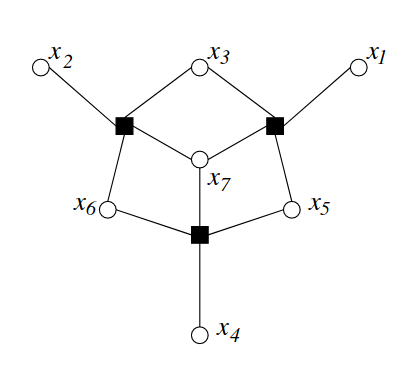
\includegraphics[width=.4\linewidth]{exmpl_1_pic_1.png}
  \captionof{figure}{factor graph for $P_0(x)$}
\end{minipage}%
\begin{minipage}[t]{.5\textwidth}
  \centering
  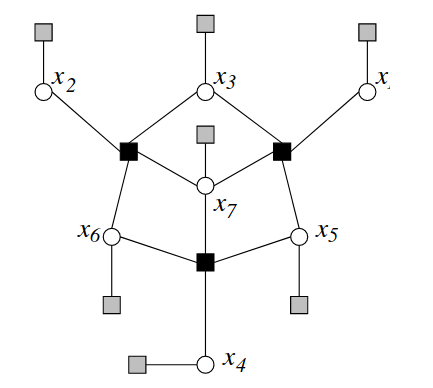
\includegraphics[width=.4\linewidth]{exmpl_1_pic_2.png}
  \captionof{figure}{factor graph for $P(x|y)$}
\end{minipage}
\end{figure}

\end{exmp}

\begin{exmp}[Edward-Anderson Model]
Consider the Edward-Anderson Model with Energy function given by $E(\sigma) = -\sum_{(i,j)}J_{ij}\sigma_i\sigma_j - B\sum_i\sigma_i$.
We can write its Boltzmann distribution as 
\EQ{\mu_\beta(\sigma) = \frac{1}{Z_\beta}\prod\limits_{\mathsmaller{(i,j)}}e^{\mathsmaller{\beta J_{ij}\sigma_i\sigma_j}}
\prod\limits_{\mathsmaller{i}}e^{\mathsmaller{\beta B\sigma_i}}}
Factor Graph for the boltzmann distribution with $L=4$ and $d=2$ is shown in Figure 3.
\begin{figure}[htb]
\centering
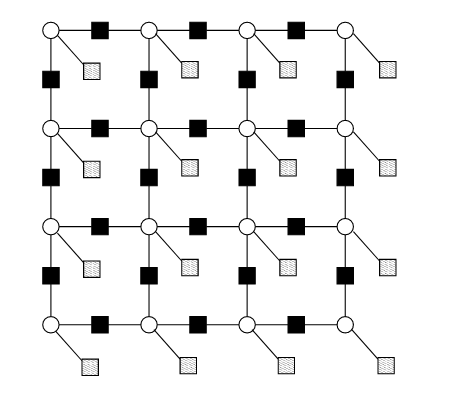
\includegraphics[width=0.25\linewidth]{exmpl_2.png}
\captionof{figure}{factor graph of $\mu_\beta$ with $L=4$ and $d=2$ }
\end{figure}
\newline
There are two types of factor nodes. Nodes corresponding to pairwise interaction terms $-J_{ij}\sigma_i\sigma_j$ in the energy function are
connected to two neighbouring variable nodes. Nodes representing magnetic field terms $-B\sigma_i$ are connected to a unique variable.
\end{exmp}

\begin{exmp}[Markov Chains]
The random variables $X_1,\dots,X_N$ taking values in the finite state space $\sX$ form a Markov Chain of order r (with $r<N$) if
\EQ{P(x_1,\dots,x_N)=P_0(x_1,\dots,x_r)\prod\limits_{t=r}^{N-1}w(x_{t-r+1}\dots x_t \to x_{t+1})} with initial conditions satisfying
\EQ{\sum\limits_{\mathsmaller{x_1\dots x_r}} P_0(x_1,\dots,x_r) = 1, \;\;\;\;\;\;\; \sum\limits_{x_0} w(x_{-r}\dots x_{-1} \to x_0) = 1.}
Factor Graph for the joint distribution with $r=2$ and $N=6$ is shown in Figure 4.
\begin{figure}[htb]
\centering
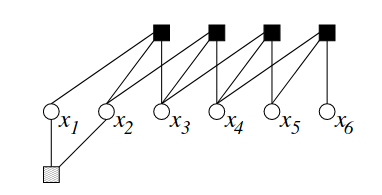
\includegraphics[width=0.25\linewidth]{exmpl_3.png}
\captionof{figure}{factor graph of $P(x_1,\dots,x_N)$ with $N=6$ and $r=2$ }
\end{figure}
\end{exmp}

\section{Sum-Product Algorithm}
The Motivation is to compute all the marginals of a global function efficiently by utilizing the structure encoded in the factor graph.
When factor graph is cycle-free, it also encodes in its structure, the arithmetic expression by which the marginals associated with the
global function may be computed.
To illustrate, we consider the following example.
\begin{exmp}
Consider the factor graph of $g(x_1,x_2,x_3,x_4,x_5) = f_A(x_1)f_B(x_2)f_C(x_1,x_2,x_3)f_D(x_3,x_4)f_E(x_3,x_5)$
\begin{figure}[htb]
\centering
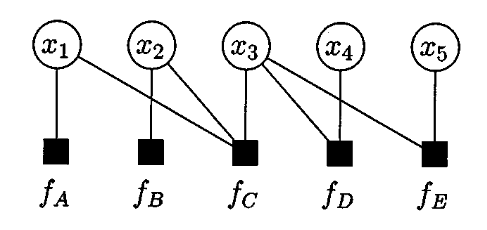
\includegraphics[width=0.25\linewidth]{exmpl_4.png}
\end{figure}
Consider computing the marginal of $x_1$
\EQ{g_1(x_1) = f_A(x_1)\left(\sum\limits_{x_2}f_B(x_2)\left(\sum\limits_{x_3}f_C(x_1,x_2,x_3)\left(\sum\limits_{x_4}f_D(x_3,x_4)\right)\left(\sum\limits_{x_5}f_E(x_3,x_5)\right)\right)\right)}
In summary notation
\EQ{g_1(x_1) = f_A(x_1)\times\sum\limits_{\sim\{x_1\}}\left(f_B(x_2)f_C(x_1,x_2,x_3)\times\left(\sum\limits_{\sim\{x_3\}}f_D(x_3,x_4)\right)\times\left(\sum\limits_{\sim\{x_3\}}f_E(x_3,x_5)\right)\right)}
Consider the Expression Tree for the above equation in Figure 5 in comparison with the factor graph redrawn as a tree with root node $x_1$
in Figure 6.
\begin{figure}[htb]
\centering
\begin{minipage}[t]{.5\textwidth}
  \centering
  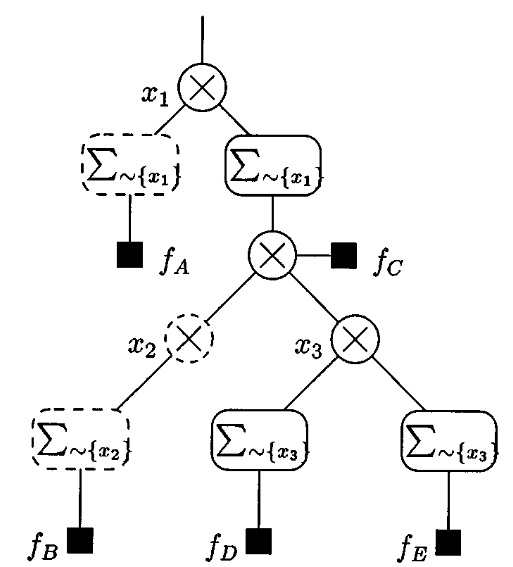
\includegraphics[width=.5\linewidth]{exmpl_5_pic_1.png}
  \captionof{figure}{expression tree for marginal of $x_1$ in $g$}
\end{minipage}%
\begin{minipage}[t]{.5\textwidth}
  \centering
  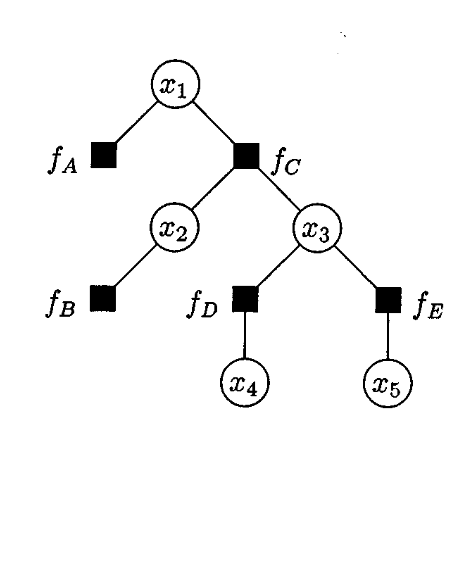
\includegraphics[width=.45\linewidth]{exmpl_5_pic_2.png}
  \captionof{figure}{factor graph redrawn with root node $x_1$}
\end{minipage}
\end{figure}
\newline
Observe that except for trivial operations, there is a one to one correspondance between expression tree for marginal of $x_1$ and factor graph
redrawn as tree with $x_1$ as root.
\end{exmp}

\begin{prop}
To convert a cycle-free graph representing a function $g(x_1,\dots,x_n)$ to corresponding expression tree for the marginal $g_i(x_i)$ of $x_i$,
draw the factor grah as a rooted tree with $x_i$ as root. Replace each variable node with a product operator. Replace each factor node with a
"form product and multiply by f" operator and between a factor node $f$ and its parent $x$, insert a $\sum\limits_{\mathsmaller{\sim\{x\}}}$ summary operator.
\end{prop}
\begin{proof}
Let $g(x,x_1,\dots,x_{N-1})$ be a function that can be represented by a cycle-free connected factor graph, \; i.e., \; a \textit{factor tree} $T$.
The Marginal or summary for x in g is $g(x) = \sum\limits_{\mathsmaller{\sim\{x\}}}g(x,x_1,\dots,x_{N-1})$.
Assuming that $x$ has $K$ neighbours in T, then without loss of generality $g$ may be written as 
\EQ{g(x,x_1,\dots,x_{N-1}) = \prod\limits_{i=1}^{K}F_i(x,X_i)}
where $F_i(x,X_i)$ is the product of all local functions in the sub-tree of T that have the $i$th neighbour of x as root and $X_i$ is the set of
variables in that subtree. Since $T$ is a tree, for $i \neq j$, $X_i \cap X_j = \emptyset$ and $X_1 \cup\dots \cup X_K = \{x_1,\dots,x_{N-1}\}$.
By distributive law,
\EQ{g(x) = \sum\limits_{\mathsmaller{\sim\{x\}}}g(x,x_1,\dots,x_{N-1}) =
\sum\limits_{X_1}\dots\sum\limits_{X_K}F_1(x,X_1)\dots F_K(x,X_K)}
\EQ{= \left(\sum\limits_{X_1}F_1(x,X_1)\right)\dots\left(\sum\limits_{X_K}F_K(x,X_K)\right) = \prod\limits_{i=1}^K\sum\limits_{\mathsmaller{\sim\{x\}}}F_i(x,X_i)}
i.e,\; \textit{the summary for $x$ in $g$ is the \textbf{product} of the summaries for $x$ of the $F_i$ function}.
\begin{figure}[htb]
\centering
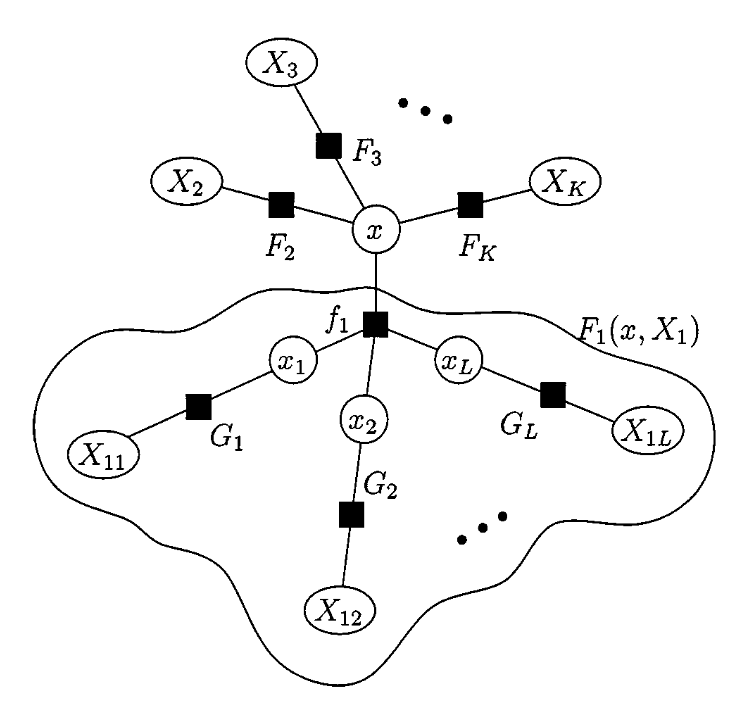
\includegraphics[width=0.4\linewidth]{exmpl_6.png}
\captionof{figure}{A generic factor tree}
\end{figure}
\newline
To compute the summary for $x$ in $F_1$, observe that, without loss of generality, $F_1(x,X_1)$ can be written as
\EQ{F_1(x,X_1) = f_1(x,x_1,\dots ,x_L)G_1(x,X_{11})\dots G_L(x_L,X_{1L})}
We note that again $\{x_1,\dots ,x_L\},X_{11},\dots,X_{1L}$ is a disjoint partition of $X_1$. Applying distributive law, we obtain
\EQ{\sum\limits_{\sim\{x\}} F_1(x,X_1) = \sum\limits_{x_1,\dots, x_L}f_1(x,x_1,\dots, x_L)\left(\sum\limits_{X_{11}}G_1(x_1,X_{11})\right)\dots\left(\sum\limits_{X_{1L}}G_L(x_L,X_{1L})\right)}

\EQ{= \sum\limits_{\sim\{x\}}\left(f_1(x_1,\dots, x_L)\prod\limits_{i=1}^L\sum\limits_{\sim\{x_i\}}G(x_i,X_{1i})\right)}
Thus, \textit{To compute the summary of $x$ in $F_1$, we should do the following : 1) for each neighbour $x_i$ of $f_1$ (other than x), compute
the summary for $x_i$ of the product of the functions in the subtree descending from $x_i$; 2) form the product of these summaries with $f_1$,
summarizing the result for $x$.}
\newline
The problem of computing the summary for $x_i$ of the product of local subtree descending from $x_i$ can be solved recursively using the same general approach.
\end{proof}

The above proposition can be easily extended into an algorithm for computing the marginal of a single variable. Start at the leaf node,
pass "unit function" if it is a variable node or pass "local function f" if it is a factor node. Each internal nodel does its operations as per
the proposition and the final marginal will be computed at the root.
Thus all the marginals can be individually computed as described above. However this is not efficient. Computation of $g_i(x_i)\; \forall i$ 
simultaneously can be efficiently accomplished by essentially "overlaying" on a single factor graph all possible instances of the above 
algorithm.
\newline
We follow the message-passing algorithm paradigm wherein each node receieves messages from neighbouring nodes, processes it and sends messages
to the other neighbouring nodes.
\paragraph{Sum-Product Algorithm}
\begin{itemize}
\renewcommand{\labelitemi}{$\Rightarrow$}
\item Initalization : Message passing is initated at leaves. If the leaf node is a variable node then "Unit function" message is passed. If the leaf node is a factor node then "local function" message is passed.
\item Update Rule : The message sent from a node $v$ on an edge $e$ is the product of the local function at $v$ (or the unit function if $v$ is 
a variable node) with all messages received at $v$ on edges other than $x$ , summarized for the variable associated with $e$.
Let $\mu_{x \to f}(x)$ denote the message sent from node $x$ to node $f$ and $\mu_{f \to x}(x)$ denote the message sent from node $f$ to node 
$x$. Let $n(v)$ denote the neighbours of node $v$. Then the update rule is given by,
\newline
\textbf{variable to local function : }
\EQ{\mu_{x \to f}(x) = \prod\limits_{\mathsmaller{h \in n(x) \setminus \{f\}}} \mu_{h \to x}(x)} 
\textbf{local function to variable : }
\EQ{\mu_{f \to x}(x) = \sum\limits_{\sim\{x\}}\left(f(n(f))\prod\limits_{\mathsmaller{y \in n(f) \setminus \{x\}}} \mu_{y \to f}(y)\right)}
\item Termination : The algorithm terminates once two messages have been passed over every edge, one in each direction.\\ At each variable node 
$x_i$, the product of all the incomming messages is the marginal function $g_i(x_i)$ of $x_i$.
\end{itemize}
\begin{figure}[htb]
\centering
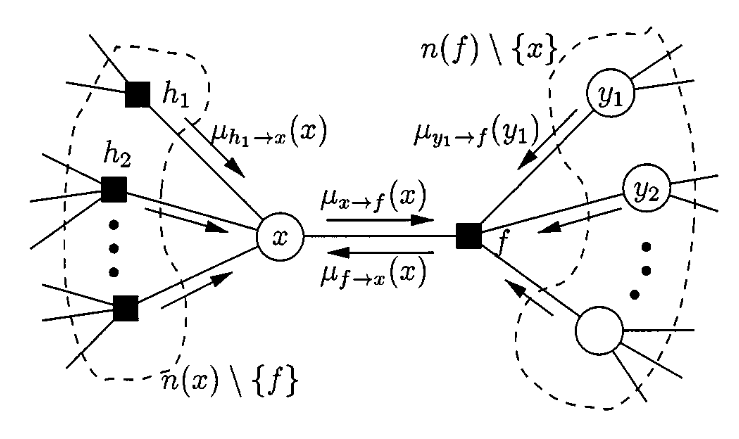
\includegraphics[width=0.6\linewidth]{exmpl_7.png}
\captionof{figure}{A factor graph fragment,showing the update rules of the sum-product algorithm }
\end{figure}
\begin{exmp}
Consider the sum-product algorithm applied to the factor graph of previous example
\begin{figure}[htb]
\centering
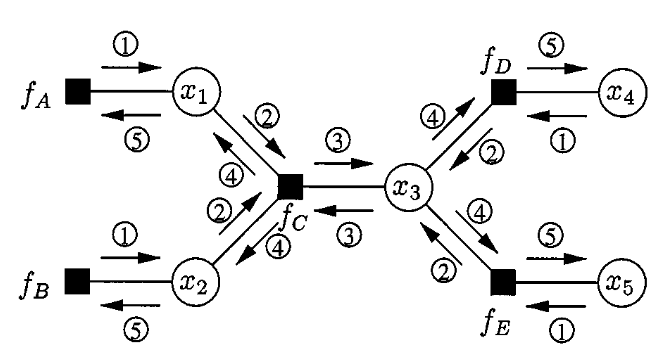
\includegraphics[width=0.5\linewidth]{exmpl_8.png}
\captionof{figure}{message generated in each step of the sum-product algorithm}
\end{figure}
\newpage
\begin{itemize}
\item Step 1 :
\EQ{\mu_{f_A \to x_1}(x_1) = \sum\limits_{\sim\{x_1\}}f_A(x_1) = f_A(x_1)}
\EQ{\mu_{f_B \to x_2}(x_2) = \sum\limits_{\sim\{x_2\}}f_B(x_2) = f_B(x_2)}
\EQ{\mu_{x_4 \to f_D}(x_4) = 1}
\EQ{\mu_{x_5 \to f_E}(x_5) = 1}
\item Step 2 :
\EQ{\mu_{x_1 \to f_C}(x_1) = \mu_{f_A \to x_1}(x_1)}
\EQ{\mu_{x_2 \to f_C}(x_2) = \mu_{f_B \to x_2}(x_2)}
\EQ{\mu_{f_D \to x_3}(x_3) = \sum\limits_{\sim\{x_3\}}\mu_{x_4 \to f_D}(x_4)f_D(x_3,x_4)}
\EQ{\mu_{f_E \to x_3}(x_3) = \sum\limits_{\sim\{x_3\}}\mu_{x_5 \to f_E}(x_5)f_D(x_3,x_5)}
\item Step 3 :
\EQ{\mu_{f_C \to x_3}(x_3) = \sum\limits_{\sim\{x_3\}}\mu_{x_1 \to f_C}(x_1)\mu_{x_2 \to f_C}(x_2)f_C(x_1,x_2,x_3)}
\EQ{\mu_{x_3 \to f_C}(x_3) = \mu_{f_D \to x_3}(x_3)\mu_{f_E \to x_3}(x_3)}
\item Step 4 :
\EQ{\mu_{f_C \to x_1}(x_1) = \sum\limits_{\sim\{x_1\}}\mu_{x_3 \to f_C}(x_3)\mu_{x_2 \to f_C}(x_2)f_C(x_1,x_2,x_3)}
\EQ{\mu_{f_C \to x_2}(x_2) = \sum\limits_{\sim\{x_2\}}\mu_{x_3 \to f_C}(x_3)\mu_{x_1 \to f_C}(x_1)f_C(x_1,x_2,x_3)}
\EQ{\mu_{x_3 \to f_D}(x_3) = \mu_{f_C \to x_3}(x_3)\mu_{f_E \to x_3}(x_3)}
\EQ{\mu_{x_3 \to f_E}(x_3) = \mu_{f_C \to x_3}(x_3)\mu_{f_D \to x_3}(x_3)}
\item Step 5 : 
\EQ{\mu_{x_1 \to f_A}(x_1) = \mu_{f_C \to x_1}(x_1)}
\EQ{\mu_{x_2 \to f_B}(x_2) = \mu_{f_C \to x_2}(x_2)}
\EQ{\mu_{f_D \to x_4}(x_4) = \sum\limits_{\sim\{x_4\}}\mu_{x_3 \to f_D}(x_3)f_D(x_3,f_4)}
\EQ{\mu_{f_E \to x_5}(x_5) = \sum\limits_{\sim\{x_5\}}\mu_{x_3 \to f_E}(x_3)f_E(x_3,f_5)}
\item Termination :
\EQ{g_1(x_1) = \mu_{f_A \to x_1}(x_1)\mu_{f_C \to x_1}(x_1)}
\EQ{g_2(x_2) = \mu_{f_B \to x_2}(x_2)\mu_{f_C \to x_2}(x_2)}
\EQ{g_3(x_3) = \mu_{f_C \to x_3}(x_3)\mu_{f_D \to x_3}(x_3)\mu_{f_E \to x_3}(x_3)}
\EQ{g_4(x_4) = \mu_{f_D \to x_4}(x_4)}
\EQ{g_5(x_5) = \mu_{f_E \to x_5}(x_5)}
\end{itemize}
\end{exmp}
\newpage
\section{Markov Random Field, Bayesian Networks and Belief Propagation}
We make connections to other graph-based language for describing probability distributions such as Markov Random Fields and Bayesian Networks.
\subsection{Markov Random Field}
\begin{defn} The Graph $G = (V,E)$ is a Markov Random Field if the distribution $P(v_1,\dots,v_n)$ satisfies local Markov Property, i.e.
\EQ{\forall v \in V \;\;\;\;\; P(v|V \setminus \{v\}) = P(v|n(v))} where n(v) denotes set of neighbours of v.
\end{defn}
A \textit{clique} in a graph is a collection of vertices which are all pairwise neighbours.
\begin{defn}
The Probability distribution $P$ is called a \textit{Gibbs Distribution} if it can be written in the factorized form
\EQ{P(v_1,\dots ,v_N) = \frac{1}{Z}\prod\limits_{E \in Q}f_E(V_E)}
where $E \subset \{1,\dots,N\}$, $Q \subset 2^N$ and $V_E \subset V$ indexed by $E$. The factors $f_E$ are called Gibbs potential functions.
\end{defn}
\begin{thm}[Hammersly-Clifford]
Let $G = (V,E)$ be a graph satisfying $p(v_1,\dots,v_N) > 0$ then $G$ is a Markov Random Field if and only if $p(v_1,\dots,v_N)$ is a Gibbs
Distribution with the set Q being the set of cliques in $G$.
\end{thm}
\begin{exmp}
Consider the distribution $p(v_1,v_2,v_3,v_4,v_5) = \frac{1}{Z}f_C(v_1,v_2,v_3)f_D(v_3,v_4)f_E(v_4,v_5)$. The corresponding markov random field
is shown in figure 10. 
\end{exmp}
\subsection{Bayesian Networks}
Bayesian Networks are graphical models for a collection of random variables that are based on Directed Acyclic Graphs(DAG).\\
Each  node $v$ in a Bayesian network is associated with a random variable. Denote by $a(v)$ the set of parents of $v$. Distribution represented
by Bayesian Network may be written as
\EQ{p(v_1,\dots ,v_N) = \prod\limits_{i=1}^N p(v_i|a(v_i)).} If $a(v_i) =\emptyset$ then $p(v_i|\emptyset) = p(v_i)$.\\
To Convert a Bayesian Network into a factor graph, simply introduce a factor node for each factor $p(v_i|a(v_i))$ and draw edges from this
node to $v_i$ and its parents $a(v_i)$.

\begin{exmp}
Consider the distribution $p(v_1,v_2,v_3,v_4,v_5) = p(v_1)p(v_2)p(v_3|v_1,v_2)p(v_4|v_3)p(v_5|v_3)$. The corresponding bayesian network
is shown in figure 11 and its factor graph is shown in figure 12.
\end{exmp}
\begin{figure}[htb]
\centering
\begin{minipage}[t]{.33\textwidth}
  \centering
  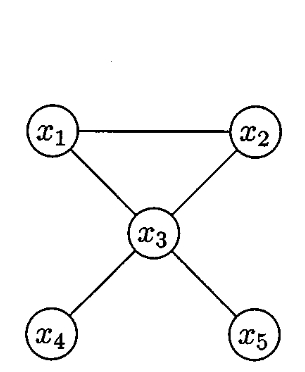
\includegraphics[width=.6\linewidth]{exmpl_9_pic_1.png}
  \captionof{figure}{}
\end{minipage}%\hfill
\begin{minipage}[t]{.33\textwidth}
  \centering
  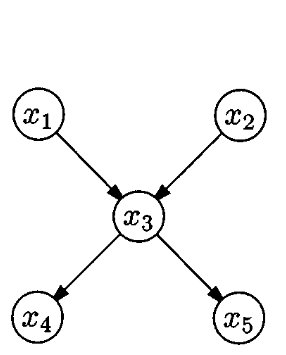
\includegraphics[width=.6\linewidth]{exmpl_9_pic_2.png}
  \captionof{figure}{}
\end{minipage}%\hfill
\begin{minipage}[t]{.33\textwidth}%
  \centering
  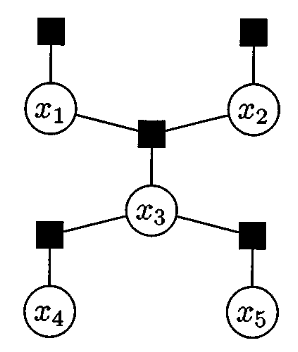
\includegraphics[width=.6\linewidth]{exmpl_9_pic_3.png}
  \captionof{figure}{}
\end{minipage}
\end{figure}
\subsection{Belief Propagation}
Belief Propagation is a message passing algorithm for performing Inference on graphical models, such as Bayesian Networks. It calculates the 
marginals for each unobserved node, conditional on any observed node. In belief propagation messages are sent between "variable nodes". Message
sent from parent $p$ to child $c$ is denoted as $\pi_c(p)$, while a message sent from $c$ to $p$ is denoted as $\lambda_c(p)$. The set of 
parents of $x$ is denoted by $a(x)$ and the set of children of $x$ is denoted by $d(x)$.
\newline
\newline
By applying the sum-product algorithm on the factor
graph corresponding to a general bayesian network, we get exactly the same update rules of the belief propagation algorithm. 
\EQ{\lambda_x(a) = \sum\limits_{\sim\{a\}}\left(\prod\limits_{d \in d(x)}\lambda_d(x)f(x|a(x))\prod\limits_{p \in a(x) \setminus \{a\}}\pi_x(p)\right) \;\;\;\;\; \forall a \in a(x)}
\EQ{\pi_d(x) = \prod\limits_{c \in d(x) \setminus \{d\}}\lambda_c(x)\sum\limits_{\sim\{x\}}\left(f(x|a(x))\prod\limits_{a \in a(x)}\pi_x(a)\right) \;\;\;\;\; \forall d \in d(x)}
The termination condition for cycle-free graphs, called the "belief update" equation is given by the product of the messages received by $x$
in the factor graph
\EQ{BEL(x) = \prod\limits_{d \in d(x)}\lambda_d(x)\sum\limits_{\sim\{x\}}\left(f(x|a(x))\prod\limits_{a \in a(x)}\pi_x(a)\right)}

\end{document}